\documentclass{beamer}

\usetheme{CambridgeUS}
\usecolortheme{beaver}
\usepackage{parskip}

\title[Fault Tolerance]{Fault Tolerance in Block-Level Caching}
\author{
  Jesus Ramos \and
  Douglas Otstott
}
\institute[FIU]{Florida International University}
\date{April 23, 2012}

\begin{document}

\maketitle

\section{Problem}

\begin{frame}
  \frametitle{Problem Statement}
  
  Fault tolerance in warehouse scale systems is an important issue
  \begin{itemize}
    \item Expect faults to happen
    \item Deal with faults online
  \end{itemize}

  Systems need to be
  \begin{itemize}
    \item Dependable and reliable
    \item Able to handle failure quickly and effectively
  \end{itemize}

\end{frame}

\section{Background}

\begin{frame}
  \frametitle{Problem Background}

  Warehouse Scale Computing Architectures utilize Storage Area
  Networks for persistent storage
  \begin{itemize}
    \item Increase reliability
    \item Easy to migrate VMs
    \item Storage Bandwidth  = \textcolor{red}{Performance Bottleneck}
  \end{itemize}

  Storage Area Networks use caches to improve throughput
  \begin{itemize}
    \item Leverages network storage
    \item Large performance increase
    \item \textcolor{red}{Reduced fault tolerance}
  \end{itemize}

\end{frame}

\begin{frame}
  \frametitle{Problem Background}
  \begin{center}
    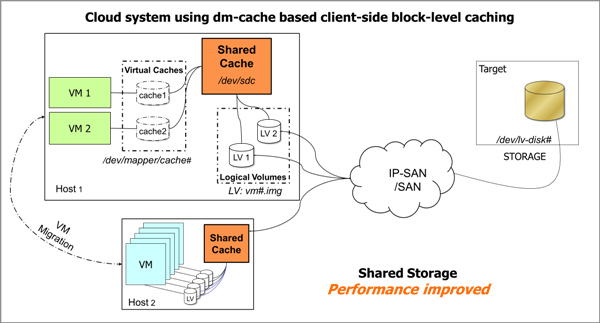
\includegraphics[scale=0.75]{../Images/NewerImage.png}
  \end{center}

  Cache device on host machine
  \begin{itemize}
    \item Virtual mapping between virtual disk and central storage
  \end{itemize}

\end{frame}

\begin{frame}
  \frametitle{DM-Cache}

  DM-Cache
  \begin{itemize}
    \item Open source block level (Linux Kernel module) caching
    solution
    \item Allows host machines to store recently used blocks
    \item Reduces the number of requests to central storage systems.
  \end{itemize}

  Increases performance
  \begin{itemize}
    \item Access time is much faster than central storage
    \item Greatly reduces contention for network storage
  \end{itemize}

  Decreases Fault Tolerance
  \begin{itemize}
    \item Metadata is non persistent
    \item Writes are buffered through the cache
    \item Local modifications are temporarily vulnerable
  \end{itemize}

\end{frame}

\section{Solution}

\begin{frame}
  \frametitle{Metadata Persistence}

  Solution:
  \begin{itemize}
    \item Move the non-persistent metadata to the persistent cache
    device
    \begin{itemize}
      \item Facilitates reconstruction of the cache
    \end{itemize}
    \item Cache the metadata in memory and write it to the cache
    device whenever it is modified after the data has been written to
    the disk
  \end{itemize}

\end{frame}

\section{Evaluation}

\begin{frame}
  \frametitle{Experimental Setup}
    
  \begin{itemize}
    \item Mtron Pro 7500 64 GB SSD
    \item iSCSI-Client: Arch Linux with Linux Kernel 3.3 running
    modified DM-Cache
    \item iSCSI-Target: Xubuntu 11.10 with 17.3GB storage target
    \item DM-Cache for 3.0 kernels
    \item IOZone I/O throughput benchmark
  \end{itemize}

\end{frame}

\graphicspath{{../Results/}}

\begin{frame}
  \frametitle{Results}
  
  \begin{center}
    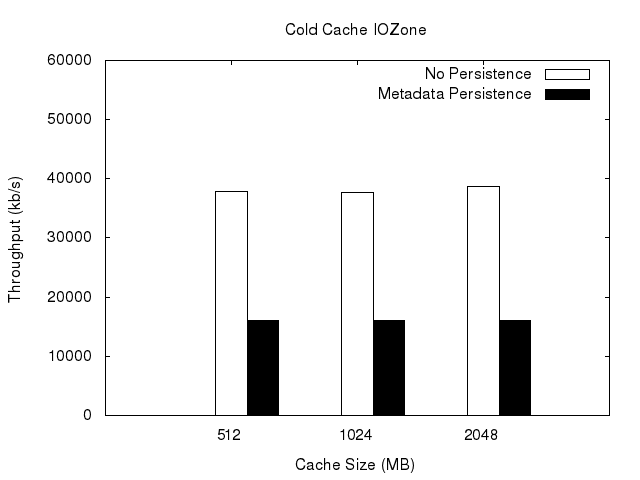
\includegraphics[scale=0.35]{results_first.png}
  \end{center}

\end{frame}

\begin{frame}
  \frametitle{Results (cont.)}

  \begin{center}
    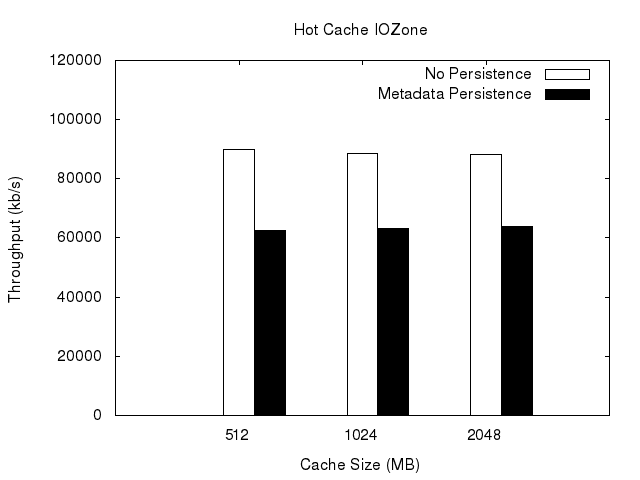
\includegraphics[scale=0.35]{results_second.png}
  \end{center}
  
\end{frame}

\begin{frame}
  \frametitle{Results Analysis}

  With a cold cache we see a 50\% reduction in throughput because
  there are a large number of modifications to the metadata on the
  disk during the warm-up period.

  Once the cache warms up the performance overhead is only about
  20-25\% because modifications to the cache happen less often.

\end{frame}

\section{Conclusion}

\begin{frame}
  \frametitle{Overhead Cost}
  
  We believe this to be a good upper-bound estimate on overhead
  costs. From evaluations of SSD performance the particular SSD brand
  we used (Mtron) is known for having very high write overhead
  compared to other SSD's.

  From preliminary testing on a Vertex SSD, which has very high
  internal write parallelism, we saw almost negligible overhead costs
  due to the added metadata writes.

\end{frame}

\begin{frame}
  \frametitle{Future Work}

  \begin{itemize}
    \item Attempt to issue the I/O's asynchronously with the data
    \item Evaluation on a broader range of SSD's
    \item More efficient ways of handling metadata writes
  \end{itemize}

\end{frame}

\section{Questions}

\begin{frame}
  \frametitle{Questions?}
  \begin{center}
    \huge ?
  \end{center}
\end{frame}

\end{document}
